%************************************************
\chapter{One Number for Two Laws}\label{ch:one-number}
%************************************************

\chapterlead{Two old laws that look like twins, a particle that carries the numbers of both, and the idea of this book.}

Pick up a pebble and let it go. It falls. Now rub a balloon on your sleeve for a few seconds and hold it close to your hair. Your hair lifts to meet it.

You have just felt the two oldest pulls in physics. The first comes from \emph{mass}. Every piece of matter pulls every other piece of matter towards it, and the Earth is simply a very large piece, so the pebble falls. The second comes from \emph{electric charge}. Rubbing moved a tiny amount of charge between your sleeve and the balloon, and charges pull on one another, or push one another away, far more fiercely than masses do. A few seconds of rubbing are enough to lift a lock of hair against the pull of the entire planet.

For more than three centuries, physics has described these two pulls with two separate laws. What is strange, and what this book is about, is how much those two laws look alike.

%------------------------------------------------
\section{Two laws with the same shape}\label{sec:two-laws}
%------------------------------------------------

\scene{Cambridge, 1687}

The first law was written down by Isaac Newton in the \emph{Principia} \citep{Newton1687,CohenWhitman1999}. Newton did not write it as an equation with a constant in front. He wrote proportions: the pull grows with the quantity of matter in each body and falls off with the square of the distance between them. The constant came later, once the world had agreed on how to measure a mass. In today's notation, and in the exact form we will use throughout this book, the gravitational force between two bodies $A$ and $B$, with masses $m_a$ and $m_b$, at a distance $r$ from each other, is
\[
\vec{F}_N = G \cdot \frac{m_a m_b}{r^2} \cdot \er .
\]
It is worth reading this slowly, one piece at a time.
\begin{itemize}
  \item $m_a m_b$ is the product of the two masses. Double one of them and the force doubles.
  \item $r^2$ is the square of the distance. Move twice as far away and the force becomes four times weaker.
  \item $G$ is the gravitational constant. It is a fixed number that nature has chosen and that we can only measure.
  \item $\er$ is an arrow of length one that points along the line joining the two bodies. It tells us in which direction the force acts.
\end{itemize}

\scene{Paris, 1785}

The second law came a century later. The French engineer Charles-Augustin de Coulomb hung a light rod from a thin wire, fixed a small charged ball to it, and measured how far the wire twisted when another charged ball came near \citep{Coulomb1785}. He faced a problem that sounds impossible: there was no instrument that could measure an amount of charge. So he invented a way around it. Touch a charged ball with an identical uncharged ball, and by symmetry the charge is shared equally between them. Touch again, and you have a quarter. Coulomb could not say how much charge there was, but he could make known fractions of it, and that was enough to find the law. In the same notation,
\[
\vec{F}_C = K \cdot \frac{q_a q_b}{r^2} \cdot \er ,
\]
where $q_a$ and $q_b$ are the two charges, measured in coulombs [C], and $K$ is the Coulomb constant.

Now put the two laws side by side, as in \Cref{fig:two-laws}. They have the same shape: a constant, times a product of two amounts, divided by the square of the distance, acting along the line between the bodies. The only differences are \emph{which} amount (mass or charge) and \emph{which} constant ($G$ or $K$).

\begin{figure}[tb]
\myfloatalign
\begin{tikzpicture}[>=Stealth, every node/.style={font=\small}]
  % ---------- Gravity panel ----------
  \begin{scope}
    \node at (1.7,1.55) {\spacedlowsmallcaps{Gravity}};
    \shade[ball color=gray!35] (0,0.35) circle (0.42);
    \shade[ball color=gray!35] (3.4,0.35) circle (0.38);
    \node at (0,0.35) {\footnotesize $m_a$};
    \node at (3.4,0.35) {\footnotesize $m_b$};
    \draw[->, very thick, Maroon] (0.5,0.35) -- (1.3,0.35);
    \draw[->, very thick, Maroon] (2.9,0.35) -- (2.1,0.35);
    \draw[|<->|, gray] (0,-0.35) -- node[below] {$r$} (3.4,-0.35);
    \node at (1.7,-1.2) {masses always attract};
    \node at (1.7,-2.05) {$\displaystyle \vec{F}_N = G \cdot \frac{m_a m_b}{r^2} \cdot \vec{e}_r$};
  \end{scope}
  % ---------- Electricity panel ----------
  \begin{scope}[xshift=6.2cm]
    \node at (1.7,1.55) {\spacedlowsmallcaps{Electricity}};
    \draw[fill=white] (0,0.75) circle (0.26) node {$+$};
    \draw[fill=white] (3.4,0.75) circle (0.26) node {$-$};
    \draw[->, very thick, Maroon] (0.35,0.75) -- (1.15,0.75);
    \draw[->, very thick, Maroon] (3.05,0.75) -- (2.25,0.75);
    \draw[fill=white] (0.8,-0.05) circle (0.26) node {$+$};
    \draw[fill=white] (2.6,-0.05) circle (0.26) node {$+$};
    \draw[->, very thick, RoyalBlue] (0.45,-0.05) -- (-0.3,-0.05);
    \draw[->, very thick, RoyalBlue] (2.95,-0.05) -- (3.7,-0.05);
    \node[align=center] at (1.7,-1.2) {opposite charges attract,\\ like charges repel};
    \node at (1.7,-2.05) {$\displaystyle \vec{F}_C = K \cdot \frac{q_a q_b}{r^2} \cdot \vec{e}_r$};
  \end{scope}
\end{tikzpicture}
\caption[Two laws with the same shape]{Two laws with the same shape. Newton's law of gravitation (left) and Coulomb's law of electrostatics (right): a constant, times a product of two amounts, divided by the square of the distance.}
\label{fig:two-laws}
\end{figure}

\paragraph{Why the square of the distance?}
There is a beautiful reason, and it is the same for both laws. Imagine something that streams out from a point in every direction without being used up, like light from a small lamp. At a distance $r$, it is spread over the surface of a sphere of area $4\pi r^2$. At twice the distance, the same total is spread over four times the area, so each small patch receives a quarter as much. Anything that spreads out this way weakens as $1/r^2$. Gravity and electricity both behave like this, which is why both laws carry the same $r^2$ underneath.

% ------------------------------------------------------------------
% Figure: why the square of the distance (Chapter 1, Section 1.1)
% Place it right after the paragraph "Why the square of the distance?"
% and end that paragraph with "... the same $r^2$ underneath
% (\Cref{fig:inverse-square})."
% Needs: tikz, pgfplots, xcolor with dvipsnames (all loaded by the book).
% ------------------------------------------------------------------
\begin{figure}[tbp]
\myfloatalign
% ================= (a) the lamp and the tiles =================
% x = distance from the lamp, y = up, z = depth (drawn slanting up and right)
\begin{tikzpicture}[>=Stealth, every node/.style={font=\small},
                    x={(1cm,0cm)}, y={(0cm,1cm)}, z={(0.8cm,0.48cm)}]
  \def\R{2.45}  % the distance r, in cm
  \def\t{0.6}   % the width of one tile, in cm

  % The bundle of light: a pyramid whose tip is the lamp.
  % Its four edges pass through the corners of every screen.
  \foreach \ya/\za/\yb/\zb in {-1/-1/1/-1, 1/-1/1/1, 1/1/-1/1, -1/1/-1/-1}
    \fill[Goldenrod!40, opacity=0.3] (0,0,0)
      -- (3*\R, {1.5*\t*\ya}, {1.5*\t*\za}) -- (3*\R, {1.5*\t*\yb}, {1.5*\t*\zb}) -- cycle;
  \foreach \yy/\zz in {-1/-1, 1/-1, 1/1, -1/1}
    \draw[Orange!80, thin] (0,0,0) -- (3*\R, {1.5*\t*\yy}, {1.5*\t*\zz});

  % Three screens, at the distances r, 2r and 3r.
  % Screen number n is n tiles wide and n tiles tall.
  % Its colour fades as 1/n^2: the same light is shared by more tiles.
  \foreach \n in {1,2,3} {
    \pgfmathsetmacro{\d}{\n*\R}          % distance of this screen
    \pgfmathsetmacro{\h}{\n*\t/2}        % half of its width
    \pgfmathsetmacro{\pct}{90/(\n*\n)}   % brightness of each tile
    \fill[Orange!\pct!white] (\d,-\h,-\h) -- (\d,\h,-\h) -- (\d,\h,\h) -- (\d,-\h,\h) -- cycle;
    \foreach \k in {1,...,\n} {          % the grid of tiles
      \draw[gray!75] (\d,{-\h+(\k-1)*\t},-\h) -- (\d,{-\h+(\k-1)*\t},\h);
      \draw[gray!75] (\d,-\h,{-\h+(\k-1)*\t}) -- (\d,\h,{-\h+(\k-1)*\t});
    }
    \draw[gray!80!black, thick] (\d,-\h,-\h) -- (\d,\h,-\h) -- (\d,\h,\h) -- (\d,-\h,\h) -- cycle;
  }

  % The lamp
  \shade[ball color=Goldenrod] (0,0,0) circle (0.17cm);
  \node[align=center, font=\footnotesize] at (0,-0.85,0) {lamp:\\ the same light\\ every second};

  % The distance axis
  \draw[->, gray] (0.3,-1.85,0) -- (3*\R+1.1,-1.85,0) node[right] {distance};
  \foreach \n/\lab in {1/r, 2/2r, 3/3r}
    \draw[gray] (\n*\R,-1.78,0) -- (\n*\R,-1.92,0) node[below] {$\lab$};

  % What each screen shows
  \node[align=center, font=\footnotesize] at (\R,2.05,0)   {$1$ tile\\ gets all the light};
  \node[align=center, font=\footnotesize] at (2*\R,2.05,0) {$2 \times 2 = 4$ tiles\\ each gets $\frac{1}{4}$};
  \node[align=center, font=\footnotesize] at (3*\R,2.05,0) {$3 \times 3 = 9$ tiles\\ each gets $\frac{1}{9}$};
\end{tikzpicture}

\par\smallskip
{\small (a) the same light, shared by more and more tiles\par}
\bigskip

% ================= (b) two spheres =================
\begin{minipage}[b]{0.36\textwidth}
\centering
\begin{tikzpicture}[>=Stealth, every node/.style={font=\footnotesize}]
  % outer sphere (radius 2r), then inner sphere (radius r), then the lamp
  \shade[ball color=Goldenrod!25, opacity=0.7] (0,0) circle (1.4cm);
  \shade[ball color=Goldenrod!75] (0,0) circle (0.7cm);
  \draw[->, thick, Maroon] (0,0) -- (-35:0.7) node[pos=0.55, above right=-1pt] {$r$};
  \draw[->, thick, RoyalBlue] (0,0) -- (215:1.4) node[pos=0.6, above left=-1pt] {$2r$};
  \fill[Orange!90!black] (0,0) circle (1.6pt);
  % the message
  \node[align=center] at (0,-1.95) {twice the radius,\\ four times the area:\\ $4\pi(2r)^2 = 4 \times 4\pi r^2$};
\end{tikzpicture}

\smallskip
{\small (b) the same light crosses both spheres\par}
\end{minipage}\hfill
% ================= (c) the same rule as a curve =================
\begin{minipage}[b]{0.6\textwidth}
\centering
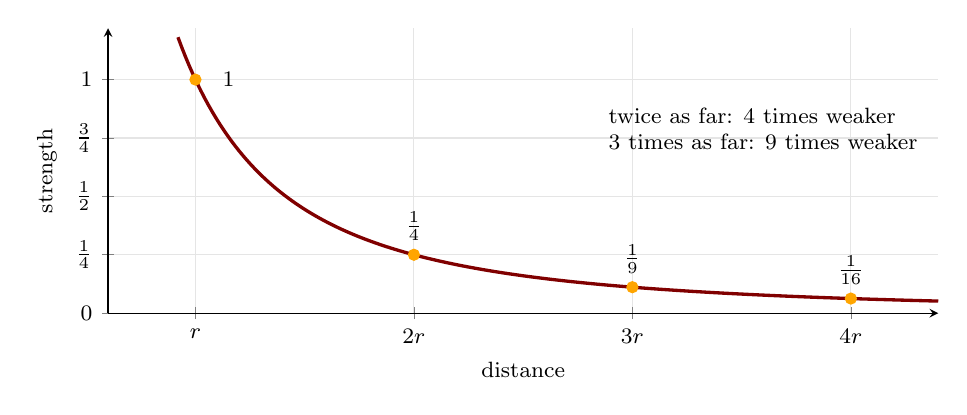
\begin{tikzpicture}
  \begin{axis}[
      width=\linewidth, height=5.2cm,
      xmin=0.6, xmax=4.4, ymin=0, ymax=1.22,
      xtick={1,2,3,4}, xticklabels={$r$,$2r$,$3r$,$4r$},
      ytick={0,0.25,0.5,0.75,1}, yticklabels={$0$,$\frac{1}{4}$,$\frac{1}{2}$,$\frac{3}{4}$,$1$},
      xlabel={distance}, ylabel={strength},
      axis lines=left, grid=major, grid style={gray!20},
      tick label style={font=\footnotesize}, label style={font=\footnotesize}]
    % the curve: strength = 1 / (distance squared)
    \addplot[very thick, Maroon, samples=200, domain=0.92:4.4] {1/x^2};
    % the points of the tiles picture
    \addplot[only marks, mark=*, mark size=2pt, Orange] coordinates {(1,1) (2,0.25) (3,0.1111) (4,0.0625)};
    \node[font=\footnotesize, anchor=west]  at (axis cs:1.08,1.0)   {$1$};
    \node[font=\footnotesize, anchor=south] at (axis cs:2,0.27)     {$\frac{1}{4}$};
    \node[font=\footnotesize, anchor=south] at (axis cs:3,0.13)     {$\frac{1}{9}$};
    \node[font=\footnotesize, anchor=south] at (axis cs:4,0.08)     {$\frac{1}{16}$};
    \node[font=\footnotesize, align=left, anchor=north east] at (axis cs:4.35,0.92)
      {twice as far: 4 times weaker\\ 3 times as far: 9 times weaker};
  \end{axis}
\end{tikzpicture}

\smallskip
{\small (c) the strength falls as $1/r^2$\par}
\end{minipage}

\caption[Why the square of the distance]{Why the square of the distance. (a) A small lamp sends out the same amount of light every second. At the distance $r$, a bundle of its rays covers one tile. At $2r$ the same rays cover a square twice as wide and twice as tall, so $2 \times 2 = 4$ tiles share the light and each receives a quarter of it. At $3r$, $3 \times 3 = 9$ tiles share it, and each receives a ninth. The fading colour shows the light growing thinner. (b) The same idea for the whole lamp: all its light crosses the sphere of radius $r$ and then the sphere of radius $2r$, whose area is four times larger. (c) The rule drawn as a curve: the strength falls from $1$ at $r$ to $\frac{1}{4}$ at $2r$, $\frac{1}{9}$ at $3r$ and $\frac{1}{16}$ at $4r$. Gravity spreads out from a mass, and the electric pull spreads out from a charge, in the same way, which is why both laws divide by $r^2$.}
\label{fig:inverse-square}
\end{figure}


\paragraph{Two important differences.}
Mass comes in only one kind, so masses always attract. Charge comes in two kinds, positive and negative: opposite charges attract and like charges repel. This is why ordinary matter hides its charge so well (positive and negative cancel out) while it can never hide its mass. The second difference is strength. Between two protons, the electric push is about $10^{36}$ times stronger than their gravitational pull. That is a one followed by thirty-six zeros, which is why a rubbed balloon can beat the whole Earth.

\paragraph{Laws need units.}
Neither law could be written with its constant until people agreed on how to measure a mass and a charge. The kilogram was first defined in 1799 through a cylinder of platinum kept in Paris, and from 1889 until 2019 the kilogram simply \emph{was} a cylinder of platinum and iridium kept near Paris. The coulomb was named in 1881 as the charge carried by a current of one ampere in one second. In 2019 both units were redefined through constants of nature: the kilogram through Planck's constant, and the coulomb by fixing the charge of a single electron exactly \citep{BIPM2019}. The value of $G$ was first reached, in effect, by Henry Cavendish in 1798, when he weighed the Earth with a twisting wire in a shed \citep{Cavendish1798}.

%------------------------------------------------
\section{One particle, two numbers}\label{sec:one-particle}
%------------------------------------------------

Now look at a single particle. An electron has a mass of about $9.109 \times 10^{-31}$ kg and a charge of about $-1.602 \times 10^{-19}$ C. A proton has a mass of about $1.673 \times 10^{-27}$ kg and a charge of $+1.602 \times 10^{-19}$ C. A neutron has almost the same mass as a proton and no charge at all.

Nature does not hand us a mass in one place and a charge in another. It hands us one particle, and the particle carries both at once. Physics, however, looks at the particle through two separate windows. Through the window of gravity it sees only the mass. Through the window of electricity it sees only the charge.

This is where the journey behind this book began. In nature a particle possesses both identifiers, its mass and its charge, while physics still approaches it from separate angles, either by its mass or by its charge. Why not by both?

So the question of this book can be stated in one sentence:
\begin{quote}
\itshape Can we write one number for a particle that holds both its mass and its charge, and one law of interaction built from that number?
\end{quote}

%------------------------------------------------
\section{The idea of this book in one line}\label{sec:idea}
%------------------------------------------------

Here is the answer this book proposes. We show it now, at the very start, so that you always know where we are going.

For a particle with mass $m$ and charge $q$, we define its \emph{cosmic mass} as
\[
\mu = m + q \cdot \Gp .
\]
It looks like an ordinary sum, but it is not one. The symbol $\Gp$ is a new kind of unit, which we call the \emph{Composer Unit}. It does not live on the number line. It points along a second axis of a new number plane, an axis that does not have to stand at a right angle to the first. The mass $m$ is measured along the first axis. The charge $q$ is counted in steps of $\Gp$ along the second axis. The Composer Unit also carries the physical unit [kg/C], kilograms per coulomb, so that $q \cdot \Gp$, just like $m$, is measured in kilograms. One number, two parts, one unit.

With one number per particle, one law can be written. For two particles with cosmic masses $\mu_a$ and $\mu_b$ at a distance $r$, the \emph{Cosmic Interaction Law} reads
\[
\vec{F}_G = G \cdot \frac{\mu_a \mu_b}{r^2} \cdot \er .
\]
It has exactly the shape of Newton's law, with cosmic masses where the masses used to be. Now multiply out the product $\mu_a \mu_b$, the way you multiply out brackets at school, and the single law opens up into three terms:
\begin{align*}
\vec{F}_G &= G \cdot \frac{m_a m_b}{r^2} \cdot \er \\
          &\quad + \Gp^2 \cdot G \cdot \frac{q_a q_b}{r^2} \cdot \er \\
          &\quad + \Gp \cdot G \cdot \frac{m_a q_b + q_a m_b}{r^2} \cdot \er .
\end{align*}
The first term is Newton's gravity. The second term pairs charge with charge, like Coulomb's law, and it is scaled by $\Gp^2$. The third term is new. It pairs the mass of each particle with the charge of the other. We call it the \emph{Coupling Force}, and it introduces a possible new fundamental interaction. Chapter~\ref{ch:interaction} shows how the law is read: by the real part of the product. Read that way, the first two terms are Newton's law and Coulomb's law, each with its full constant, and the Coupling Force has no real part, so it adds nothing to the force along the line between the two particles.

\begin{plainwords}
What to take away from this section:
\begin{itemize}
  \item one number per particle, the cosmic mass $\mu$, with a mass part and a charge part;
  \item one law, shaped like Newton's law, written with cosmic masses;
  \item three terms inside that law: gravity, a Coulomb-like term, and a new coupling term;
  \item one way to read that law, by its real part: it gives Newton's law and Coulomb's law exactly, and the coupling term adds no force between the two particles.
\end{itemize}
Do not worry yet about what $\Gp$ really is. Chapter~\ref{ch:general-numbers} builds it from the ground up.
\end{plainwords}

Two words of fairness before we go on. First, what you have just read is a proposal, not an established result of physics. Every step that leads to it will be stated clearly, so that you can follow it and judge it for yourself. Second, the symbol $\Gp$ is doing a great deal of work in those two lines, and it deserves a proper introduction. It will get one.

Chapter~\ref{ch:alignment} comes first. It says how a new theory is judged, by the old laws it must give back and by the new results it must predict, and it gathers what this volume shows. To build the law itself, we need to travel in four steps:
\begin{enumerate}
  \item Chapter~\ref{ch:oblique} frees the triangle from its right angle. This gives us the \emph{General Sinus}, a sine and a cosine with two variables.
  \item Chapter~\ref{ch:general-numbers} frees the number plane from its right angle. This gives us the \emph{General Numbers} and the Composer Unit $\Gp$.
  \item Chapter~\ref{ch:prologue} explains why the language of physics must sometimes grow, and what this book does and does not try to do.
  \item Chapter~\ref{ch:interaction} puts mass and charge into the new number plane and derives the Cosmic Interaction Law.
\end{enumerate}
But first, a short walk through the history of numbers. It will show us that what we are about to do has been done before, several times, and always in the same way.

%------------------------------------------------
\section{How numbers grow}\label{sec:numbers-grow}
%------------------------------------------------

Have you ever seen a three? Not three goats, and not the symbol 3 printed on a page, but three itself? Nobody has. Numbers live in a world of ideas, and yet they fit the real world astonishingly well. How did we come to have them?

\scene{Border Cave, southern Africa, about 43{,}000 years ago}

Before there were numbers, there were notches. A small bone found at Border Cave, in the Lebombo Mountains on today's border between eSwatini and South Africa, carries twenty-nine notches cut by a human hand \citep{dErrico2012}. The Ishango bone, found near Lake Edward in today's Democratic Republic of the Congo and some twenty to twenty-five thousand years old, carries marks arranged in groups \citep{BrooksSmith1987}. We do not know what they counted. We do know the idea behind them: someone decided that a mark could stand for a thing, one mark for one goat, one mark for one day. Everything that follows in this book is that same decision, taken again and again at higher and higher stakes.

Later, something even more important happened, and nobody wrote down when. People noticed that three fish and three days share something, and that this something can be named on its own. That shared thing is the number three. Once numbers came loose from the things they counted, they could be carried anywhere, combined, and argued about.

From there, numbers grew. And they grew in a very particular way: each time, a simple question was asked that the numbers of the time could not answer.
\begin{itemize}
  \item \emph{What is $3 - 5$?} With only counting numbers, there is no answer. The Chinese calculators of the Han period used red and black counting rods for amounts owned and amounts owed \citep{Shen1999}. In India in 628, Brahmagupta wrote down rules for fortunes and debts, and treated zero as a number in its own right \citep{Colebrooke1817,Plofker2009}. The answer to the question was a new kind of number: the negative numbers.
  \item \emph{What is $1 \div 3$?} The answer needed fractions, which Egyptian and Babylonian scribes had used for thousands of years.
  \item \emph{How long is the diagonal of a square whose side is $1$?} Its square is $2$, and the Greeks discovered that no fraction whatsoever has a square equal to $2$. Legend says the discovery cost a man named Hippasus his life. The legend is almost certainly a later decoration, but the shock was real. The answer was a new kind of number: the irrational numbers, such as $\sqrt{2}$.
  \item \emph{Which number, multiplied by itself, gives $-1$?} Every number on the line gives a positive result when squared. The answer was the strangest new number of all.
\end{itemize}

\Cref{tab:ladder-small} gathers these steps. Read from top to bottom, it is a ladder, and each rung was built because someone refused to accept that a reasonable question had no answer.

\begin{table}[tb]
\myfloatalign
\begin{tabularx}{\textwidth}{@{}l c >{\raggedright\arraybackslash}X@{}}
\toprule
\tableheadline{The question} & & \tableheadline{The new numbers} \\
\midrule
How many? & $\mathbb{N}$ & counting numbers $1, 2, 3, \dots$ \\
What is $3 - 5$? & $\mathbb{Z}$ & negative numbers and zero \\
What is $1 \div 3$? & $\mathbb{Q}$ & fractions \\
Which number squares to $2$? & $\mathbb{R}$ & irrational numbers such as $\sqrt{2}$ \\
Which number squares to $-1$? & $\mathbb{C}$ & complex numbers \\
\bottomrule
\end{tabularx}
\caption[The ladder of numbers]{The ladder of numbers. Each new kind of number answered a question that the old numbers could not: $\mathbb{N} \subset \mathbb{Z} \subset \mathbb{Q} \subset \mathbb{R} \subset \mathbb{C}$.}
\label{tab:ladder-small}
\end{table}

\scene{Milan, 1545, and Bologna, 1572}

The last question arrived in the middle of a quarrel between Italian mathematicians over how to solve equations. In 1545 Gerolamo Cardano set a problem of schoolboy simplicity: divide ten into two parts whose product is forty \citep{Cardano1545}. Calling the parts $x$ and $10 - x$, the algebra gives
\[
x\,(10 - x) = 40 \quad\Longrightarrow\quad x^2 - 10x + 40 = 0 \quad\Longrightarrow\quad x = 5 \pm \sqrt{-15}.
\]
There is no such pair of ordinary numbers; the largest product you can get by splitting ten is twenty-five. Yet Cardano noticed that if he multiplied the two impossible answers together, obeying the usual rules, he got exactly forty. He called the exercise as subtle as it was useless, and moved on.

Twenty-seven years later, Rafael Bombelli, an engineer who drained marshes for a living, met a case he could not walk away from \citep{Bombelli1572}. The equation $x^3 = 15x + 4$ has the perfectly ordinary solution $x = 4$, as you can check. But the standard formula of the day produced
\[
x = \sqrt[3]{2 + \sqrt{-121}} + \sqrt[3]{2 - \sqrt{-121}} .
\]
Bombelli had what he called a wild thought. What if these strange cube roots were numbers of the form ``two plus something impossible'' and ``two minus the same thing''? Writing $i$ for the unit whose square is $-1$ (so that $\sqrt{-121} = 11i$), he found
\[
(2 + i)^3 = 2 + 11i, \qquad (2 - i)^3 = 2 - 11i,
\]
so the two cube roots are $2 + i$ and $2 - i$, and their sum is exactly $4$. The impossible numbers were not a sign that the question was wrong. They were the only road to the right answer.

Still, they were not welcome. René Descartes called them \emph{imaginary} in 1637, and he did not mean it kindly \citep{Descartes1637}. They took another two centuries to become respectable.

\paragraph{The freedom to define.}
How can anyone simply decide that a number whose square is $-1$ exists? Two teachers at the University of Cape Town explain it to their students in a way worth keeping: in mathematics we are free to define new objects, as long as they do not contradict the rules we already have, and then we discover what our definitions commit us to \citep{MokhithiShock2020}. Nobody discovered $i$ lying on the ground. Somebody defined it. What they could not choose were its consequences, and the consequences turned out to be wonderful.

%------------------------------------------------
\section{The quarter turn}\label{sec:quarter-turn}
%------------------------------------------------

So what \emph{is} $i$? The clearest answer is a picture, and it is the picture this whole book grows from \citep{MokhithiShock2020,Needham1997}.

Think of the number line. Adding a number moves you to the right or to the left. Multiplying by $2$ stretches you away from zero. Multiplying by $-1$ flips you to the other side of zero. Now try a puzzle: which single step, done twice, takes you from $1$ to $-1$? Stretching never crosses zero. Flipping twice brings you back to where you started. On the line, there is no such step.

In a plane, there is. Turn a quarter of a full turn, counterclockwise, around zero. The number $1$ moves to a point one unit \emph{above} zero. Turn once more and you arrive at $-1$. That halfway point is $i$ (\Cref{fig:quarter-turn}). Multiplying by $i$ is a quarter turn, and the famous rule $i^2 = -1$ says nothing more mysterious than this: two quarter turns make a half turn.
% ------------------------------------------------------------------
% Figure: three moves on the number line (Chapter 1, Section 1.5)
% Place it right after the paragraph that begins "Think of the number line."
% and add "(\Cref{fig:number-line})" after "... flips you to the other side of zero".
% Needs: tikz and xcolor with dvipsnames (both loaded by the book).
% ------------------------------------------------------------------
\begin{figure}[tbp]
\myfloatalign
\begin{tikzpicture}[>=Stealth, x=1.12cm, every node/.style={font=\small}]

  % A number line from -4 to 4, drawn at height #1
  \newcommand{\drawnumberline}[1]{%
    \draw[->, gray] (-4.6,#1) -- (4.7,#1);
    \foreach \k in {-4,...,4} {
      \draw[gray] (\k,#1+0.07) -- (\k,#1-0.07);
      \node[below, font=\footnotesize, gray!80!black] at (\k,#1-0.07) {$\k$};
    }
  }

  % ================= (a) adding: slide =================
  \begin{scope}[yshift=0cm]
    \node[anchor=west, font=\small\bfseries] at (-4.6,2.3) {(a) adding: slide along the line};
    \drawnumberline{0}
    % adding 2 to 1: two steps to the right
    \draw[->, very thick, Maroon] (1,0.12) to[out=70, in=110]
      node[above, font=\footnotesize, align=center] {$1 + 2 = 3$\\ two steps right} (3,0.12);
    % adding -3 to 1: three steps to the left
    \draw[->, very thick, Maroon!60] (1,0.12) to[out=110, in=70]
      node[above, font=\footnotesize, align=center] {$1 + (-3) = -2$\\ three steps left} (-2,0.12);
    \fill[Maroon] (1,0) circle (2.2pt);
    \draw[Maroon, fill=white, thick] (3,0) circle (2.2pt);
    \draw[Maroon!60, fill=white, thick] (-2,0) circle (2.2pt);
  \end{scope}

  % ================= (b) multiplying by 2: stretch =================
  \begin{scope}[yshift=-3.2cm]
    \node[anchor=west, font=\small\bfseries] at (-4.6,1.75) {(b) multiplying by $2$: stretch away from zero};
    \drawnumberline{0}
    % each number moves to twice its distance from zero, on the same side
    \draw[->, very thick, RoyalBlue] (1,0.12)  to[out=75, in=105] (2,0.12);
    \draw[->, very thick, RoyalBlue] (2,0.12)  to[out=65, in=115] (4,0.12);
    \draw[->, very thick, RoyalBlue] (-1,0.12) to[out=105, in=75] (-2,0.12);
    \draw[->, very thick, RoyalBlue] (-2,0.12) to[out=115, in=65] (-4,0.12);
    \foreach \x in {1,2,-1,-2} \fill[RoyalBlue] (\x,0) circle (2.2pt);
    \node[font=\footnotesize, RoyalBlue] at (1.5,0.68)  {$1 \to 2$};
    \node[font=\footnotesize, RoyalBlue] at (3,1.12)    {$2 \to 4$};
    \node[font=\footnotesize, RoyalBlue] at (-1.5,0.68) {$-1 \to -2$};
    \node[font=\footnotesize, RoyalBlue] at (-3,1.12)   {$-2 \to -4$};
    % zero does not move
    \fill (0,0) circle (2.4pt);
    \node[font=\footnotesize, align=center] at (0,0.75) {$0$ stays\\ where it is};
  \end{scope}

  % ================= (c) multiplying by -1: flip =================
  \begin{scope}[yshift=-7.3cm]
    \node[anchor=west, font=\small\bfseries] at (-4.6,2.85) {(c) multiplying by $-1$: flip to the other side of zero};
    \drawnumberline{0}
    % zero acts as a mirror
    \draw[dashed, gray] (0,-0.05) -- (0,2.2) node[above, font=\footnotesize, black] {mirror at $0$};
    % nested arches over zero: each number lands at the same distance, on the other side
    \draw[->, very thick, ForestGreen] (1,0.12) .. controls (1,0.76) and (-1,0.76) .. (-1,0.12);
    \draw[->, very thick, ForestGreen!70!black] (-2,0.12) .. controls (-2,1.49) and (2,1.49) .. (2,0.12);
    \draw[->, very thick, ForestGreen] (3,0.12) .. controls (3,2.23) and (-3,2.23) .. (-3,0.12);
    \foreach \x in {1,-2,3} \fill[ForestGreen] (\x,0) circle (2.2pt);
    \node[font=\footnotesize, fill=white, inner sep=1pt, text=ForestGreen!70!black] at (0,0.86) {$1 \to -1$};
    \node[font=\footnotesize, fill=white, inner sep=1pt, text=ForestGreen!70!black] at (0,1.42) {$-2 \to 2$};
    \node[font=\footnotesize, fill=white, inner sep=1pt, text=ForestGreen!70!black] at (1.25,1.93) {$3 \to -3$};
  \end{scope}
\end{tikzpicture}
\caption[Three moves on the number line]{Three moves on the number line. (a) Adding slides you along the line: adding $2$ takes $1$ to $3$, two steps to the right, and adding $-3$ takes $1$ to $-2$, three steps to the left. (b) Multiplying by $2$ stretches the whole line away from zero: $1$ goes to $2$ and $2$ goes to $4$, $-1$ goes to $-2$ and $-2$ goes to $-4$. Every number ends up twice as far from zero, on the same side, and zero itself does not move. (c) Multiplying by $-1$ flips the line around zero, as in a mirror: $1$ goes to $-1$, $-2$ goes to $2$ and $3$ goes to $-3$. Every number keeps its distance from zero and changes side. Flip twice, and you are back where you started.}
\label{fig:number-line}
\end{figure}
\begin{figure}[tb]
\myfloatalign
\begin{tikzpicture}[scale=1.55, >=Stealth, every node/.style={font=\small}]
  \draw[->, gray] (-1.7,0) -- (1.8,0) node[right] {real};
  \draw[->, gray] (0,-1.55) -- (0,1.7) node[above] {imaginary};
  \draw[gray!40] (0,0) circle (1);
  \foreach \pt/\lab/\pos in {{(1,0)}/{$1$}/{below right}, {(0,1)}/{$i$}/{above right}, {(-1,0)}/{$-1$}/{below left}, {(0,-1)}/{$-i$}/{below right}}
    { \fill[Maroon] \pt circle (1.3pt) node[\pos] {\lab}; }
  \draw[->, very thick, Maroon] (5:1.12) arc (5:85:1.12) node[pos=0.5, above right] {$\times\, i$};
  \draw[->, very thick, Maroon] (95:1.12) arc (95:175:1.12) node[pos=0.5, above left] {$\times\, i$};
  \draw[->, thick, RoyalBlue, dashed] (-5:0.8) arc (-5:-85:0.8);
  \draw[->, thick, RoyalBlue, dashed] (-95:0.8) arc (-95:-175:0.8);
  \node[RoyalBlue] at (-0.55,-0.95) {$\times\,(-i)$};
\end{tikzpicture}
\caption[The quarter turn]{The quarter turn. Multiplying by $i$ turns a number by a quarter of a full turn around zero; two quarter turns carry $1$ to $-1$. Turning the other way, by $-i$, also reaches $-1$ in two steps.}
\label{fig:quarter-turn}
\end{figure}

Keep turning, and the powers of $i$ go round in a cycle of four:
\[
i^1 = i, \qquad i^2 = -1, \qquad i^3 = -i, \qquad i^4 = 1 .
\]
Each power adds one more quarter turn: $90^\circ$, $180^\circ$, $270^\circ$, and finally $360^\circ$, back where we started. Remember this cycle. We will meet it again in Chapter~\ref{ch:general-numbers}, wearing new clothes.

\scene{Copenhagen, 1797}

This picture was first drawn by a Norwegian surveyor working in Denmark, Caspar Wessel. He spent his days turning bearings and distances into maps, which meant adding and combining directions. In a paper presented in 1797, whose title means \emph{On the Analytical Representation of Direction}, he showed that if you describe a direction by a length and an angle, then the rule ``multiply the lengths and add the angles'' behaves exactly like multiplication \citep{Wessel1799}. His paper went almost unnoticed for a hundred years. Jean-Robert Argand found the same picture in 1806 \citep{Argand1806}, and Carl Friedrich Gauss, who had kept it to himself for decades, published it in 1831 with all his authority and gave these numbers the name they still carry: not imaginary, but \emph{complex} \citep{Gauss1831}. In 1837 William Rowan Hamilton removed the last mystery by showing that a complex number is simply an ordered pair of real numbers with a clear rule for multiplying pairs \citep{Hamilton1837}.

So a complex number $a + bi$ is a point of the plane: $a$ steps along the real axis and $b$ steps along the imaginary axis. Multiplying two complex numbers multiplies their lengths and adds their angles. For numbers of length one, written with the angles $\alpha$ and $\beta$, this rule reads
\[
(\cos\alpha + i \sin\alpha)(\cos\beta + i\sin\beta) = \cos(\alpha + \beta) + i\sin(\alpha + \beta),
\]
and it is nothing other than the addition formulas for sine and cosine that astronomers had used for sixteen centuries to follow the Moon. Leonhard Euler packed the whole story into one line, $e^{i\theta} = \cos\theta + i\sin\theta$ \citep{Euler1748}. And in 1893 the engineer Charles Proteus Steinmetz showed that alternating currents can be computed with complex numbers, because the phase of a current is an angle, and multiplying by a complex number adds an angle \citep{Steinmetz1893}. Every power grid on Earth is designed that way today.

% ------------------------------------------------------------------
% Figure: multiplying turns, and the old rule of the sky (Chapter 1, Section 1.5)
% Place it right after the paragraph that ends "... to follow the Moon. ..."
% and add "(\Cref{fig:moon-rule})" after "... to follow the Moon".
% Needs: tikz and xcolor with dvipsnames (both loaded by the book).
% ------------------------------------------------------------------
\begin{figure}[tbp]
\myfloatalign
% ================= (a) multiplying turns: the angles add =================
\begin{minipage}[b]{0.47\textwidth}
\centering
\begin{tikzpicture}[>=Stealth, scale=1.75, every node/.style={font=\footnotesize}]
  \def\a{50}  % angle of the first number
  \def\b{25}  % angle of the second number
  \draw[->, gray] (-0.3,0) -- (1.3,0) node[below left] {real};
  \draw[->, gray] (0,-0.15) -- (0,1.02);
  \draw[gray!50] (1,0) arc (0:115:1);
  % the two numbers and their product, all of length one
  \draw[RoyalBlue] (0,0) -- (\b:1);
  \draw[Maroon] (0,0) -- (\a:1);
  \draw[very thick, Plum] (0,0) -- ({\a+\b}:1);
  % the angle of the product: first alpha, then beta on top of it
  \draw[Maroon, thick] (0.3,0) arc (0:\a:0.3);
  \node[Maroon] at (37:0.43) {$\alpha$};
  \draw[RoyalBlue, thick] (\a:0.3) arc (\a:{\a+\b}:0.3);
  \node[RoyalBlue] at ({\a+\b/2}:0.43) {$\beta$};
  % multiplying by the second number turns the first one by beta
  \draw[->, thick, Plum] (\a+4:1.12) arc (\a+4:{\a+\b-4}:1.12);
  \node[Plum, anchor=south west] at (62:1.15) {turn by $\beta$};
  \fill[RoyalBlue] (\b:1) circle (1.3pt) node[right] {angle $\beta$};
  \fill[Maroon] (\a:1) circle (1.3pt) node[right] {angle $\alpha$};
  \fill[Plum] ({\a+\b}:1) circle (1.5pt);
  \node[Plum, anchor=south east, align=right] at (0.24,1.03) {product:\\ angle $\alpha + \beta$};
\end{tikzpicture}

\smallskip
{\footnotesize $(\cos\alpha + i\sin\alpha)(\cos\beta + i\sin\beta)$\\
$= \cos(\alpha + \beta) + i\sin(\alpha + \beta)$\\[2pt]
for any lengths: the lengths multiply, the angles add\par}

\smallskip
{\small (a) multiplying: the angles add\par}
\end{minipage}\hfill
% ================= (b) following the Moon =================
\begin{minipage}[b]{0.5\textwidth}
\centering
\begin{tikzpicture}[>=Stealth, every node/.style={font=\footnotesize}]
  \def\R{1.75}  % radius of the Moon's path (taken as one unit)
  \def\a{35}    % today's angle of the Moon
  \def\b{13}    % the Moon moves about 13 degrees in a day (drawn to scale)
  \draw[gray!60, dashed] (0,0) circle (\R);
  \draw[->, gray] (0,0) -- (2.35,0) node[below right=-2pt, align=left] {starting\\ direction};
  \draw[->, gray] (0,0) -- (0,2.15);
  % where tomorrow's Moon stands: how far across and how far up
  \draw[gray, dashed] ({\a+\b}:\R) -- ({\R*cos(\a+\b)},0);
  \draw[gray, dashed] ({\a+\b}:\R) -- (0,{\R*sin(\a+\b)});
  \node[below] at ({\R*cos(\a+\b)/2},0) {$\cos(\alpha + \beta)$};
  \node[left]  at (0,{\R*sin(\a+\b)/2}) {$\sin(\alpha + \beta)$};
  % today's angle alpha, then one day's step beta
  \draw[Maroon, thick] (0.55,0) arc (0:\a:0.55);
  \node[Maroon] at ({\a/2}:0.75) {$\alpha$};
  \draw[RoyalBlue, thick] (\a:0.95) arc (\a:{\a+\b}:0.95);
  \node[RoyalBlue] at ({\a+\b/2}:1.17) {$\beta$};
  % the Earth and two positions of the Moon
  \shade[ball color=RoyalBlue!55] (0,0) circle (0.17);
  \node[left=4pt] at (0,0) {Earth};
  \shade[ball color=gray!25] (\a:\R) circle (0.11);
  \shade[ball color=gray!25] ({\a+\b}:\R) circle (0.11);
  \node[anchor=west] at (\a-4:\R+0.15) {today};
  \node[anchor=south west] at ({\a+\b+2}:\R+0.1) {tomorrow};
  \node[RoyalBlue, anchor=north west, align=left] at (1.25,-1.15) {$\beta \approx 13^\circ$:\\ one day's step};
\end{tikzpicture}

\smallskip
{\footnotesize $\sin(\alpha + \beta) = \sin\alpha\cos\beta + \cos\alpha\sin\beta$\\
$\cos(\alpha + \beta) = \cos\alpha\cos\beta - \sin\alpha\sin\beta$\\[2pt]
tables give $\alpha$ and $\beta$, the rule gives $\alpha + \beta$\par}

\smallskip
{\small (b) following the Moon\par}
\end{minipage}

\bigskip
% ================= (c) sixteen centuries of the same rule =================
\begin{tikzpicture}[>=Stealth, every node/.style={font=\footnotesize, align=center}]
  % the year y is drawn at x = 1.35 + (y - 150) * 8.5 / 1647 cm
  \draw[->, thick, gray] (0.3,0) -- (11.0,0);
  \foreach \y/\lab/\pos in {150/{c.\ 150\\ Ptolemy, Alexandria\\ a table of chords}/above,
                            499/{499\\ Aryabhata, India\\ half-chords: our sines}/below,
                            980/{about 980\\ Abu al-Wafa, Baghdad\\ the sine of a sum}/above,
                            1464/{1464\\ Regiomontanus\\ brings it to Europe}/below,
                            1797/{1797\\ Wessel, Copenhagen\\ it multiplies numbers}/above}
  {
    \pgfmathsetmacro{\x}{1.35+(\y-150)*8.5/1647}
    \fill[Maroon] (\x,0) circle (2pt);
    \node[\pos=3pt] at (\x,0) {\lab};
  }
  \draw[decorate, decoration={brace, amplitude=5pt, mirror}, gray]
    (1.35,-1.45) -- (9.85,-1.45) node[midway, below=6pt, text=black] {about sixteen centuries of the same addition rule};
\end{tikzpicture}

\smallskip
{\small (c) from the chords of Ptolemy to the numbers of Wessel\par}

\caption[Multiplying turns, and an old rule of the sky]{Multiplying turns, and an old rule of the sky. (a) On the circle of radius one, the number at angle $\alpha$ times the number at angle $\beta$ lands at angle $\alpha + \beta$: multiplying by the second number turns the first one by $\beta$. For numbers of other lengths, the lengths multiply as well. (b) Astronomers met the same rule when they followed the Moon. The Moon moves about $13^\circ$ a day against the stars, so tomorrow's angle is today's angle $\alpha$ plus one day's step $\beta$. To turn the new angle into a position, how far across and how far up, they needed the sine and the cosine of a sum, and the addition formulas give these from the values for $\alpha$ and for $\beta$, which they read from their tables. (c) The same rule, first written with chords and later with sines, served astronomers from Ptolemy to Wessel, about sixteen centuries, until Wessel's picture showed that it is also the rule for multiplying numbers.}
\label{fig:moon-rule}
\end{figure}

% ------------------------------------------------------------------
% Figure and box: alternating current with complex numbers (Chapter 1, Section 1.5)
% Place them right after the paragraph that mentions Steinmetz (1893), and end its
% last sentence with "... designed that way today (\Cref{fig:steinmetz})."
% Needs: tikz, xcolor with dvipsnames and the plainwords box (all in the book).
% ------------------------------------------------------------------
\begin{figure}[tbp]
\myfloatalign
% ================= (a) a current is a turning arrow =================
\begin{tikzpicture}[>=Stealth, every node/.style={font=\footnotesize}]
  \def\r{1.1}     % length of the arrow: the peak current I_0
  \def\th{50}     % the angle of the arrow at this moment
  \def\L{6.0}     % one full turn of the arrow = this many cm of time
  % the circle and the turning arrow
  \draw[gray!50] (0,0) circle (\r);
  \draw[gray] (-1.35,0) -- (1.35,0);
  \draw[->, very thick, RoyalBlue] (0,0) -- (\th:\r) node[midway, above left=-2pt] {$I_0$};
  \draw[RoyalBlue] (0.35,0) arc (0:\th:0.35);
  \node[RoyalBlue, anchor=west] at (0.4,0.17) {$\omega t + \phi$};
  \draw[->, gray] (110:1.3) arc (110:150:1.3);
  \node[align=center] at (0,-1.55) {the arrow turns\\ $50$ times a second};
  % the wave traced by the height of the tip
  \draw[->, gray] (2.0,0) -- (2.0+\L+0.5,0) node[right] {time};
  \draw[very thick, RoyalBlue!80, smooth, domain=0:360, samples=120, variable=\t]
    plot ({2.0+\t/360*\L}, {\r*sin(\t)});
  \draw[dashed, gray] (\th:\r) -- ({2.0+\th/360*\L}, {\r*sin(\th)});
  \fill[RoyalBlue] ({2.0+\th/360*\L}, {\r*sin(\th)}) circle (1.6pt);
  \node[anchor=south west, align=left] at (2.0+0.55*\L, 0.1)
    {the height of the tip\\ is the current:\\ $I(t) = I_0 \sin(\omega t + \phi)$};
\end{tikzpicture}

\par\smallskip
{\small (a) an alternating current is a turning arrow, and its phase is an angle\par}
\bigskip

% ================= (b) multiplying by Z turns the arrow =================
\begin{tikzpicture}[>=Stealth, every node/.style={font=\footnotesize}]
  % ---------- resistor: Z = R, no turn ----------
  \begin{scope}
    \draw[thick] (-0.6,1.75) -- (-0.35,1.75) -- (-0.25,1.9) -- (-0.05,1.6) -- (0.15,1.9) -- (0.35,1.6) -- (0.45,1.75) -- (0.7,1.75);
    \draw[->, very thick, Maroon] (0,0.07) -- (1.3,0.07) node[above] {$\hat{V}$};
    \draw[->, very thick, RoyalBlue] (0,-0.07) -- (0.9,-0.07) node[below] {$\hat{I}$};
    \node[align=center] at (0.35,-1.6) {resistor: $Z = R$\\ no turn: $\hat{V}$ in step with $\hat{I}$};
  \end{scope}
  % ---------- coil: Z = i omega L, +90 degrees ----------
  \begin{scope}[xshift=3.9cm]
    \draw[thick] (-0.6,1.75) -- (-0.4,1.75) arc (180:0:0.1) arc (180:0:0.1) arc (180:0:0.1) arc (180:0:0.1) arc (180:0:0.1) -- (0.7,1.75);
    \draw[->, very thick, RoyalBlue] (0,0) -- (0.9,0) node[below] {$\hat{I}$};
    \draw[->, very thick, Maroon] (0,0) -- (0,1.2) node[right] {$\hat{V}$};
    \draw[gray] (0.4,0) arc (0:90:0.4);
    \node at (45:0.65) {$+90^\circ$};
    \node[align=center] at (0.35,-1.6) {coil: $Z = i\omega L$\\ a quarter turn ahead};
  \end{scope}
  % ---------- capacitor: Z = 1/(i omega C), -90 degrees ----------
  \begin{scope}[xshift=7.8cm]
    \draw[thick] (-0.6,1.75) -- (0.0,1.75); \draw[thick] (0.0,1.53) -- (0.0,1.97);
    \draw[thick] (0.13,1.53) -- (0.13,1.97); \draw[thick] (0.13,1.75) -- (0.7,1.75);
    \draw[->, very thick, RoyalBlue] (0,0) -- (0.9,0) node[above] {$\hat{I}$};
    \draw[->, very thick, Maroon] (0,0) -- (0,-1.0) node[right] {$\hat{V}$};
    \draw[gray] (0.4,0) arc (0:-90:0.4);
    \node at (-45:0.68) {$-90^\circ$};
    \node[align=center] at (0.35,-1.6) {capacitor: $Z = 1/(i\omega C)$\\ a quarter turn behind};
  \end{scope}
\end{tikzpicture}

\par\smallskip
{\small (b) $\hat{V} = Z\,\hat{I}$: multiplying by $Z$ turns the arrow\par}

\caption[Alternating current with complex numbers]{Alternating current with complex numbers. (a) An alternating current is the height of an arrow of length $I_0$ that turns at a steady rate, $50$ times a second on the electricity grids of Morocco and Europe. The angle of the arrow is the phase of the current. (b) In a circuit, the voltage across each part is the current multiplied by a complex number $Z$, called the impedance. A resistor multiplies by a real number and leaves the angle as it is. A coil multiplies by $i\omega L$, which turns the voltage a quarter turn ahead of the current. A capacitor multiplies by $1/(i\omega C)$, which turns it a quarter turn behind. Multiplying by a complex number adds its angle: this is why Steinmetz could compute alternating currents with complex numbers.}
\label{fig:steinmetz}
\end{figure}

\paragraph{Two readings, one number.}
Connect any device to the mains, a lamp, a motor or a phone charger, and measure it with two instruments. A voltmeter tells you how hard the electricity is being pushed, in volts. An ammeter tells you how much of it flows, in amperes. With alternating current both readings swing back and forth fifty times a second, and they do not always swing together: in a coil the push reaches its peak a quarter of a swing before the flow does, and in a capacitor a quarter of a swing after it. So the relation between the two readings holds two facts, not one. The first is a size: how many volts it takes to drive one ampere through the device. The second is a delay: how far the swing of the voltage runs ahead of, or behind, the swing of the current.

Steinmetz kept both facts in a single complex number, the \emph{impedance} $Z$. Its length is the size, measured in ohms, which are volts per ampere. Its angle is the delay. Write the voltage and the current as turning arrows, that is, as complex numbers $\hat{V}$ and $\hat{I}$, and the whole relation becomes one division:
\[
Z = \frac{\hat{V}}{\hat{I}} = \frac{V_0}{I_0}\,e^{i(\phi_V - \phi_I)} = R + iX .
\]
The last form tells the same story in another way. Its real part $R$ is the \emph{resistance}: the share of the electrical energy that the device turns into heat and light, as a toaster or a lamp does. Its imaginary part $X$ is the \emph{reactance}: the energy that coils and capacitors store during part of each swing and then give back. Two different physical behaviours, measured in the same unit, travel together in one number, and the rules of complex arithmetic do all the bookkeeping. Multiply a current by $Z$, and out comes the voltage, with its size and its delay already right.

\begin{plainwords}[The impedance as one complex number]
\begin{itemize}
  \item Voltage and current as turning arrows: $\hat{V} = V_0\,e^{i\phi_V}$ and $\hat{I} = I_0\,e^{i\phi_I}$.
  \item The impedance is their ratio, $Z = \hat{V}/\hat{I} = |Z|\,e^{i\theta}$, with the size $|Z| = V_0/I_0$ in ohms and the angle $\theta = \phi_V - \phi_I$, the delay between the two swings.
  \item The same number in two parts: $Z = R + iX$, with the resistance $R = |Z|\cos\theta$ and the reactance $X = |Z|\sin\theta$. Back again: $|Z| = \sqrt{R^2 + X^2}$ and $\tan\theta = X/R$.
  \item A resistor, a coil and a capacitor in a row give $Z = R + iX$ with $X = \omega L - \dfrac{1}{\omega C}$.
\end{itemize}
\end{plainwords}

\paragraph{What else belongs in one number?}
The impedance invites a bolder question. If two facts that seemed to need two separate lines, a size and a delay, can live together in one number, are there other notions of physics that belong together in the same way? The first candidates are the ones we met at the start of this chapter. Every particle carries a mass and a charge. They are measured with different instruments and in different units, kilograms and coulombs, and they enter two different laws that nevertheless have exactly the same shape (\Cref{sec:two-laws}). Could they, too, be written as one number, as the cosmic mass $\mu = m + q \cdot \Gp$ of \Cref{sec:idea} proposes?

And if they can, which kind of number should hold them? History advises us not to take the answer for granted. Look again at the questions of \Cref{tab:ladder-small}. With the counting numbers alone, $3 - 5$ has no answer: someone had to make the negative numbers. The division $1 \div 3$ needed the fractions. A number whose square is $2$ needed the irrational numbers. A number whose square is $-1$ needed the complex numbers. Each time the question first looked impossible, and each time the way out was not to drop the question but to enlarge the numbers, keeping all the old ones inside the new. So the question for mass and charge has two halves. Can they share one number? And are the complex numbers, with their two axes fixed at a right angle, the right home for them, or is it time, once again, for a new kind of number?



%------------------------------------------------


\begin{plainwords}[What we have so far]
\begin{itemize}
  \item Gravity and electricity obey two laws with the same shape, and every particle carries the numbers of both: a mass and a charge.
  \item This book proposes one number for both, the cosmic mass $\mu = m + q \cdot \Gp$, and one law built from it, which opens into three terms.
  \item Numbers grow when a reasonable question has no answer. The last great step gave us $i$, the quarter turn.
  \item The complex plane is built on a right angle. The rest of the book asks what happens when that right angle is set free.
\end{itemize}
\end{plainwords}
